\section{Entwicklungsstand IT-Jobs}
Zum Zeitpunkt der Beendigung dieser Arbeit sind folgende Teilmodule abgeschlossen:
\begin{itemize}
 \item Modul: \glossar{CMS}. Blog und statische Seiten sowie die Möglichkeit variablen Inhalt auf beliebigen Seiten innerhalb der Sidebar darzustellen
 \item Modul: Job, Basis. Implementation des Datenbank\index{Datenbank}schemas für Jobs und die Möglichkeit Jobs über das Interface anzulegen
 \item Modul: Feedimport. Möglichkeit, Jobs mittels einer XML-Schnittstelle in das System einzuspielen. E-Mail Benachrichtigung im Fehlerfalle an den Inhaber der XML-Feeds
\end{itemize}
Noch offen für eine zukünftige Entwicklung sind:
\begin{itemize}
 \item Modul: Bewerbung. Bewerber können sich über die Webseite bewerben. Ebenfalls können sie sich mit Facebook und LinkedIn verbinden, um automatisch ihre Stammdaten eintragen zu lassen
 \item Modul: Bezahlsystem: Beim Anlegen eines Jobs wird dieser über einen externen Dienstleister abgewickelt.
\end{itemize}

Während der Arbeiten an IT-Jobs\index{IT-Jobs-Projekt} wurden andere Aufgaben priorisiert und deswegen der Abgabetermin für das System nach 2012 verlegt. Nichtsdestotrotz soll IT-Jobs als Basistechnologie und Referenzprojekt für weitere Rails\index{Ruby-on-Rails}-Anwendungen dienen und die Entwicklung kann insgesamt als Erfolg bewertet werden, auch wenn sie zum gegenwärtigen Zeitpunkt noch nicht abgeschlossen ist.

An der Entwicklung beteiligt waren 2 Programmierer, einschließlich des Autors. Beiden Programmierern gelang es, sich mit der Testgetriebene\index{TDD}n Entwicklung und mit Rails\index{Ruby-on-Rails} vertraut zu machen und wertvolle Erfahrungen zu sammeln.

\subsection*{Code-Qualität und Testabdeckung}
Während der Entwicklung wurden in regelmäßigen Abständen Code-Metrik\index{Code-Metrik}en festgehalten und können nun so über den Verlauf der Entwicklung dargestellt werden.

\begin{figure}[htbp]
 \centering
 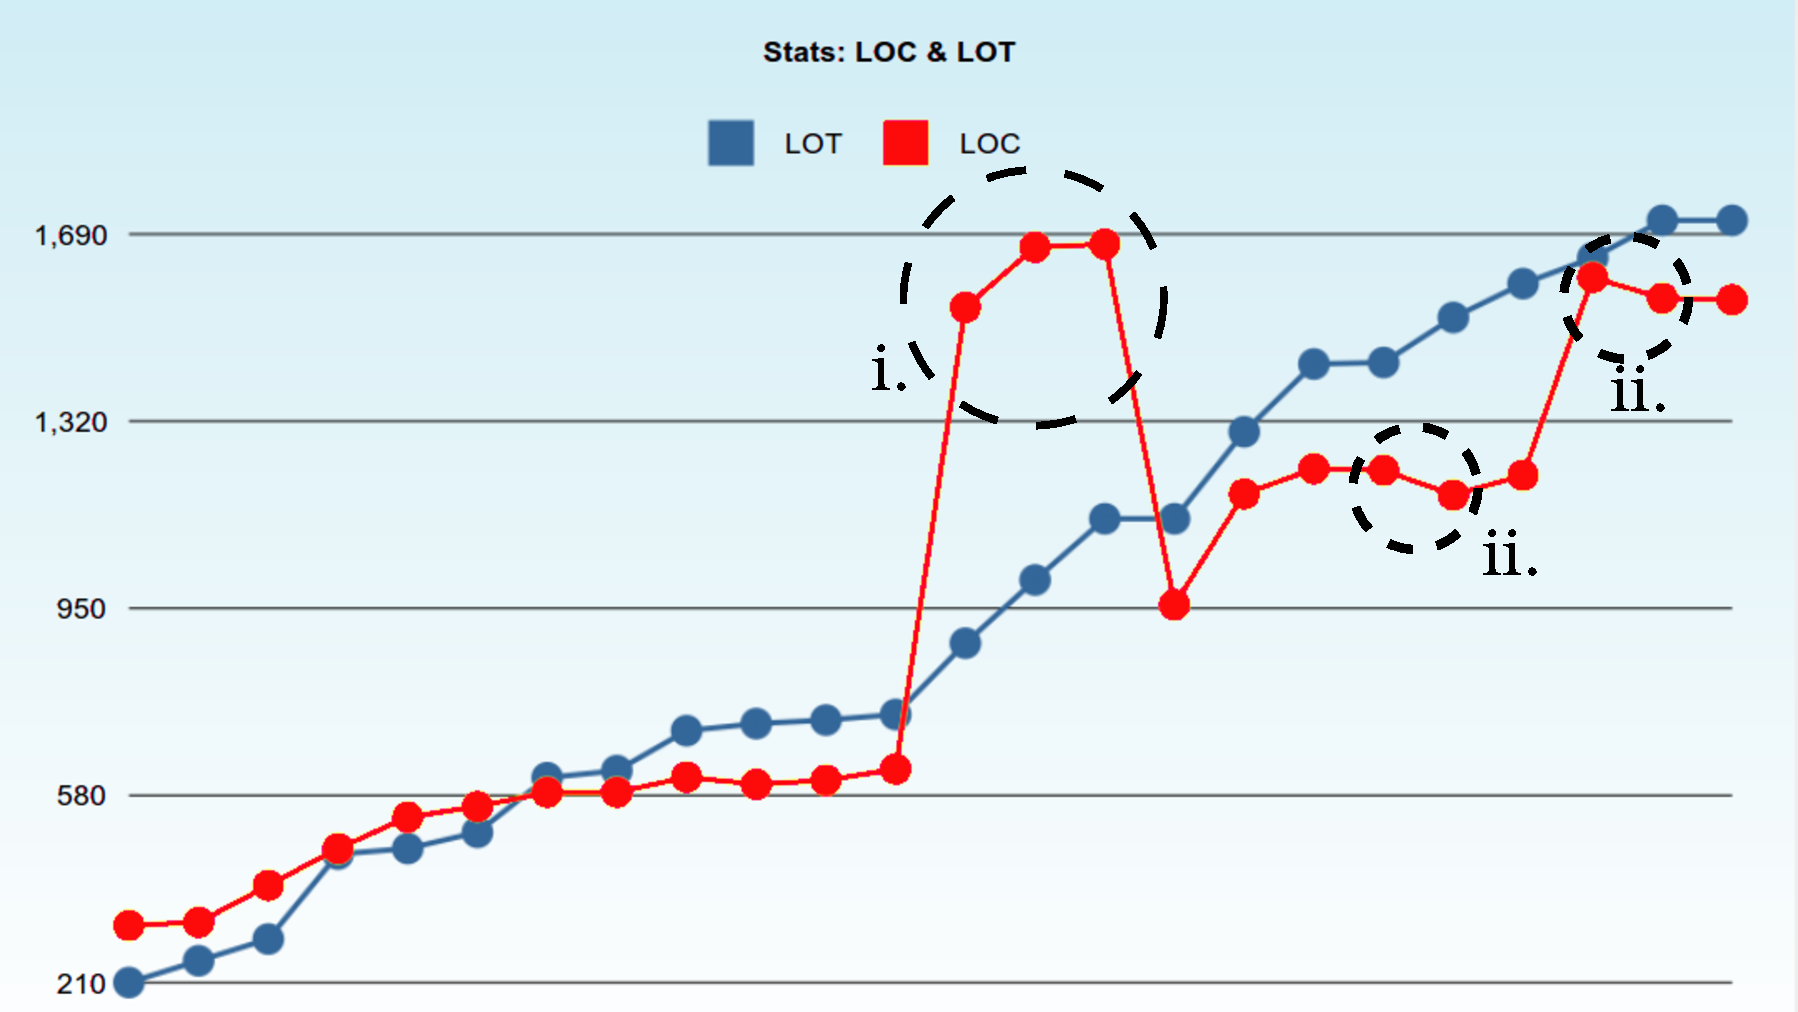
\includegraphics[width=0.9\textwidth]{./diagrams/itjobs-loclot.pdf}
 % itjobs-loclot.png: 1000x600 pixel, 72dpi, 35.28x21.17 cm, bb=0 0 1000 600
 \caption{Entwicklung des Umfangs des Test- und Programmcodes}
 \label{fig:itjobsLoc}
\end{figure}

In Abbildung \ref{fig:itjobsLoc} ist der Verlauf der Codezeilen und der Testzeilen abgebildet. Während in den ersten Tagen der Entwicklung, wegen dem Einsatzes von Codegenerator\index{Code-Generator}en und einer langsamen Gewöhnung an den TDD\index{TDD} Ablauf, noch weniger Testcode als Programmcode geschrieben wurde, verlaufen die Linien ab dann nahezu proportional. Einen Ausreißer stellen die mit i. markierte Codezeilen dar: Hier ist eine Fehlkonfiguration der Statistikberechnung die Ursache dafür, dass Fremdcode mitgezählt wurde, der nicht Teil der Anwendung war. Eine andere interessante Erkenntnis ist, dass zwar die Lines Of Test \index{Test}monoton steigend ist, die Lines Of Code dagegen durch Refaktorisierung\index{Refaktorisierung}en abgefallen sind (z.B. mit ii. markierte Stellen). Die hohe Testdichte hat eine Refaktoriserung ermöglicht und in diesen Phasen konnte effektiv Design zu dem System hinzugefügt werden.


\begin{figure}[htbp]
 \centering
 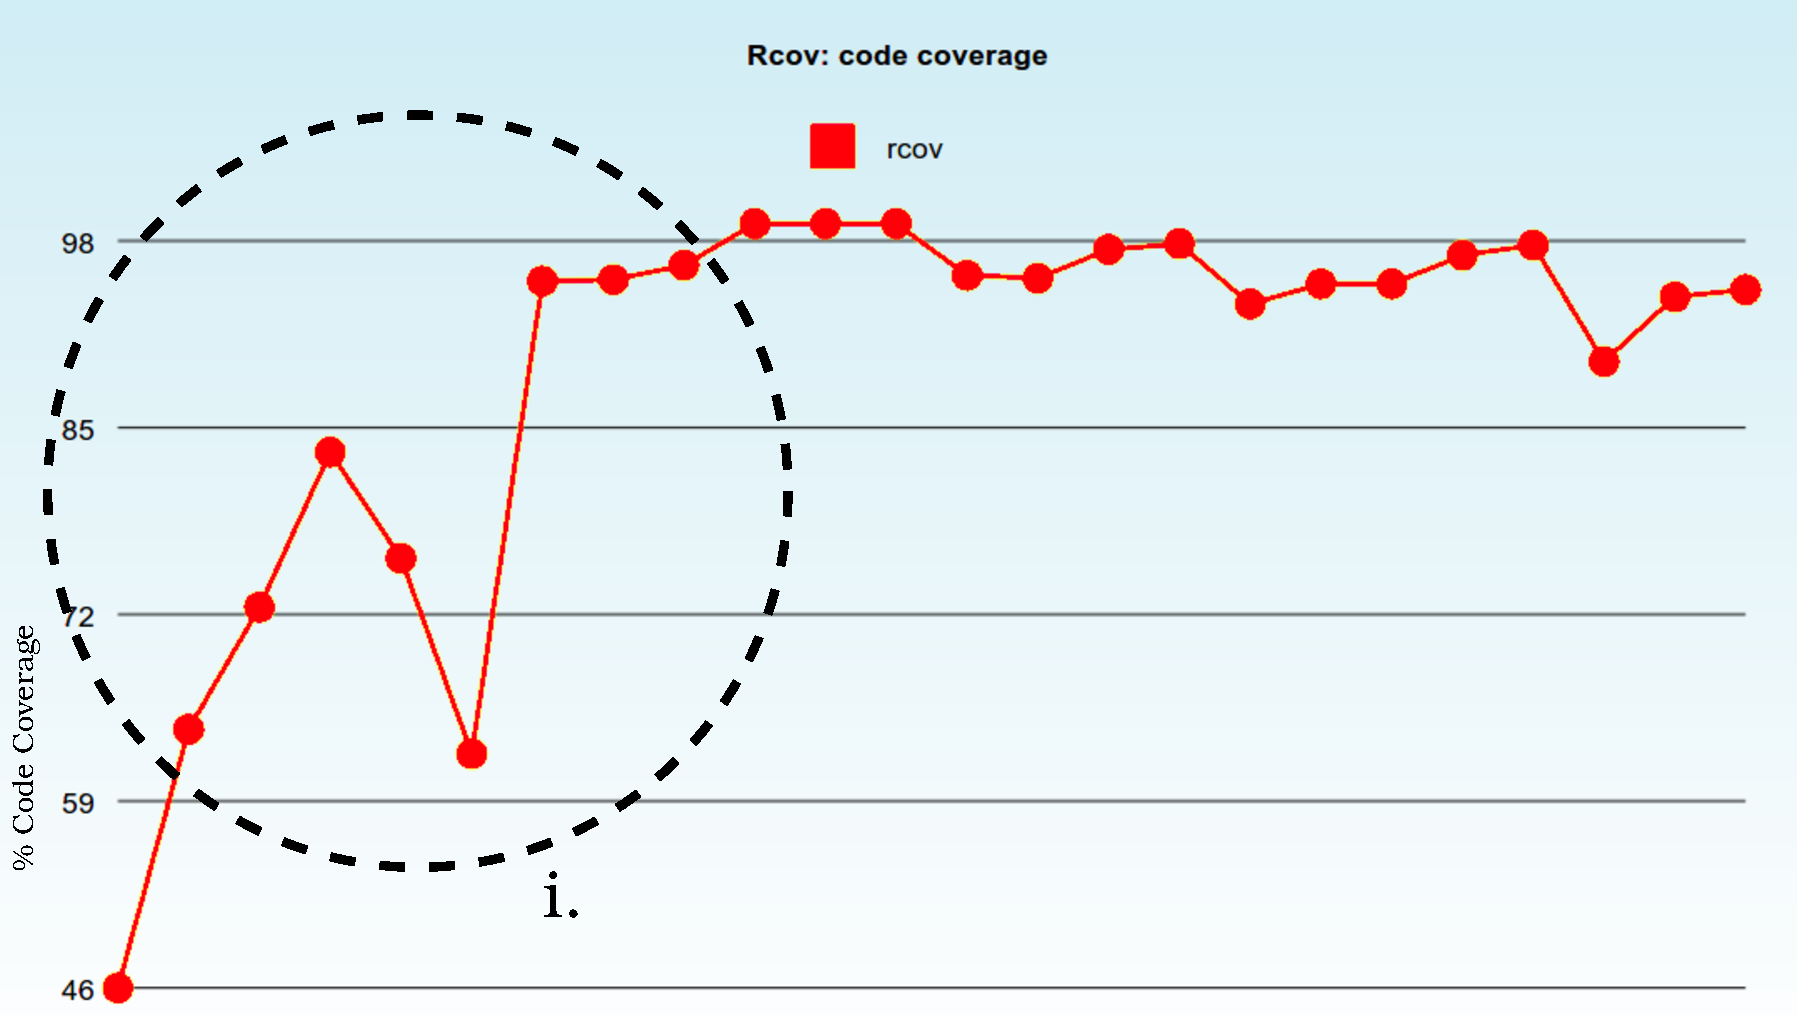
\includegraphics[width=\textwidth]{./diagrams/itjobs-coverage.pdf}
 % itjobs-coverage.pdf: 862x487 pixel, 72dpi, 30.41x17.18 cm, bb=
 \caption{C0-Testabdeckung über den Verlauf der Entwicklung}
 \label{fig:itjobsCoverage}
\end{figure}
In Abbildung \ref{fig:itjobsCoverage} ist der Verlauf der \glossar{Testabdeckung}\index{Test!Testabdeckung} über den Verlauf der Entwicklung abgebildet. Insbesondere in den ersten Tagen gab es einige Probleme, die davon verursacht wurden, dass das Tool mit dem die Abdeckung gemessen wurde, "`rcov"' nicht kompatibel mit der aktuellen Ruby Version 1.9.2 ist. RCov lieferte deshalb falsche Werte liefert. Später erfolgte eine Umstellung auf SimpleCov (bereits in Abschnitt \ref{sec:devtools} vorgestellt). Ab dann lag die Testabdeckung innerhalb von 90\% bis 100\%.

\begin{figure}[htbp]
 \centering
 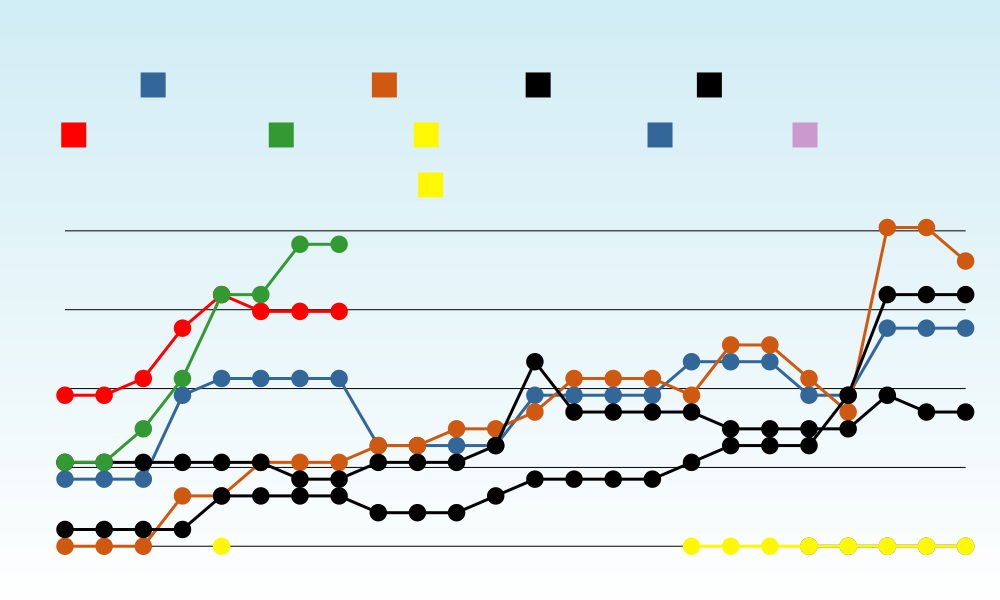
\includegraphics[width=\textwidth]{./diagrams/itjobs-smells.png}
 % itjobs-coverage.pdf: 862x487 pixel, 72dpi, 30.41x17.18 cm, bb=
 \caption{Verlauf der verschiedenen Klassen an Code-Smells über den Entwicklungszeitraum}
 \label{fig:itjobsSmells}
\end{figure}

Ein Indikator für die Code-Qualität sind die Anzahl und Arten von Code-Smell\index{Code-Smell}s. Diese wurden ebenfalls über den Entwicklungszeitraum gemessen und sind in Abbildung \ref{fig:itjobsSmells} dargestellt. Insgesamt betrachtet, stiegen diese mit zunehmender Codemenge langsam an. Dank der Messung durch Code-Metrik\index{Code-Metrik}en konnte einige suboptimale Stellen nach einer gewissen Zeit refaktorisiert werden. So ist das wiederkehrende Muster, dass die Anzahl der Vorkommen eines Codesmells erst anstieg und nach einigen Tagen wieder abfiel. Das Ergebnis gilt als positiv zu bewerten, da die Menge an Code-Smells langsamer anstieg, als die dazugehörige Menge an Code (LOC, vgl. Abbildung \ref{fig:itjobsLoc}). Die Code-Smells wurden mit dem Werkzeug Reek gemessen und die Definition der Code-Smells sowie Informationen über das jeweilige Messverfahren entnehmen sie bitte \citep{kevin_rutherford_code_2010}.

\subsection*{Diskussion}
Falls das Projekt in einem reinen TDD\index{TDD}-Vorgehen entwickelt worden wäre, dann hätte die Testabdeckung\index{Test!Testabdeckung} 100\% betragen müssen. Ist war aber nicht immer der Fall. Gründe hierfür sind:
\begin{itemize}
 \item Nutzung von Codegenerator\index{Code-Generator}en. Bei der Erstellung der Gerüste und der Programmierung einfacher Administrationsinterfaces waren nicht immer Testfälle mitgeneriert worden. Stellenweise wurde dieser generierte Code später neu in TDD\index{TDD} geschrieben, allerdings nicht in allen Fällen
 \item Vorher waren schon einige Erfahrung mit Rails\index{Ruby-on-Rails} vorhanden. Allerdings sind in der neusten Version von Rails einige Features dazu gekommen und wurden nun einige Bibliotheken verwendet, die vorher noch nicht bekannt waren. Aus der Unkenntnis entstand so viel Code, der eigentlich zum Experimentieren mit diesen neuen Features gedacht war. Diese Spikes (siehe Abschnitt \ref{sec:tddspecialcircumstances}) dienen dem Erkunden neuer Funktionalitäten und dem Prototypisieren. Diese sollten normalerweise nicht in den Hauptzweig der Entwicklung mit eingecheckt werden. In zukünftigen Projekten, die nach dem Prinzip der kontinuierlichen Integration stattfinden werden (siehe Abschnitt \ref{sec:auswahlWeitere}), wird ein Einchecken dieser Spikephasen in den Hauptzweig der Entwicklung nicht erfolgen.
 \item Trotz bisheriger Erfahrungen mit Ruby und Rails\index{Ruby-on-Rails} waren nur wenig Erfahrungen zum Thema Testen und Testgetriebene\index{TDD} Entwicklung vorhanden. Insbesondere die Nutzung von \glossarpl{Test-Double}\index{Test-Double} musste erst gelernt werden, da ohne eine solche bestimmte Testszenarien schwierig bis überhaupt nicht zu testen sind.
\end{itemize}

Trotzdem ermöglichte die vorhande Testdichte eine sichere Ausgangsbasis für ständige Refaktorisierung\index{Refaktorisierung}en. Ein Ergebnis dessen ist, dass die Anzahl der Code-Smell\index{Code-Smell}s im akzeptablen Rahmen geblieben ist. Eine gewisse Menge an Komplexität lässt sich nicht vermeiden und Code-Smells können hier nur ein Indikator sein. In vielen Fällen muss direkt am Code entschieden werden, ob ein gewisser Code-Smell für eine gewisse Stelle relevant ist oder nicht.
